\documentclass[12pt]{beamer}
\usepackage{../Estilos/BeamerFC}
\usepackage{../Estilos/ColoresLatex}
\usepackage{courier}
\usepackage{listingsutf8}
\usepackage{listings}
\usepackage{xcolor}
\usepackage{textcomp}
\usepackage{color}
\definecolor{deepblue}{rgb}{0,0,0.5}
\definecolor{brown}{rgb}{0.59, 0.29, 0.0}
\definecolor{OliveGreen}{rgb}{0,0.25,0}
% \usepackage{minted}

\DeclareCaptionFont{white}{\color{white}}
\DeclareCaptionFormat{listing}{\colorbox{gray}{\parbox{0.98\textwidth}{#1#2#3}}}
\captionsetup[lstlisting]{format=listing,labelfont=white,textfont=white}
\renewcommand{\lstlistingname}{Código}


\definecolor{Code}{rgb}{0,0,0}
\definecolor{Keywords}{rgb}{255,0,0}
\definecolor{Strings}{rgb}{255,0,255}
\definecolor{Comments}{rgb}{0,0,255}
\definecolor{Numbers}{rgb}{255,128,0}

\makeatletter

\newif\iffirstchar\firstchartrue
\newif\ifstartedbyadigit
\newif\ifprecededbyequalsign

\newcommand\processletter
{%
  \ifnum\lst@mode=\lst@Pmode%
    \iffirstchar%
        \global\startedbyadigitfalse%
      \fi
      \global\firstcharfalse%
    \fi
}

\newcommand\processdigit
{%
  \ifnum\lst@mode=\lst@Pmode%
      \iffirstchar%
        \global\startedbyadigittrue%
      \fi
      \global\firstcharfalse%
  \fi
}

\lst@AddToHook{OutputOther}%
{%
  \lst@IfLastOtherOneOf{=}
    {\global\precededbyequalsigntrue}
    {}%
}

\lst@AddToHook{Output}%
{%
  \ifprecededbyequalsign%
      \ifstartedbyadigit%
        \def\lst@thestyle{\color{orange}}%
      \fi
    \fi
  \global\firstchartrue%
  \global\startedbyadigitfalse%
  \global\precededbyequalsignfalse%
}

\lstset{ 
language=Python,                % choose the language of the code
basicstyle=\footnotesize\ttfamily,       % the size of the fonts that are used for the code
numbers=left,                   % where to put the line-numbers
numberstyle=\scriptsize,      % the size of the fonts that are used for the line-numbers
stepnumber=1,                   % the step between two line-numbers. If it is 1 each line will be numbered
numbersep=5pt,                  % how far the line-numbers are from the code
backgroundcolor=\color{white},  % choose the background color. You must add \usepackage{color}
showspaces=false,               % show spaces adding particular underscores
showstringspaces=false,         % underline spaces within strings
showtabs=false,                 % show tabs within strings adding particular underscores
frame=single,   		% adds a frame around the code
tabsize=2,  		% sets default tabsize to 2 spaces
captionpos=t,   		% sets the caption-position to bottom
breaklines=true,    	% sets automatic line breaking
breakatwhitespace=false,    % sets if automatic breaks should only happen at whitespace
escapeinside={| |},  % if you want to add a comment within your code
stringstyle =\color{OliveGreen},
otherkeywords={as, np.array, np.concatenate, np.linspace, linspace, interpolate.interp1d, kind, plt.plot, .copy, np.arange, np.cos, np.pi, lw, ls, label, splrep, splev, plt.legend, loc, plt.title, plt.ylim, plt.show, sign, math.ceil, math.log, np.sqrt, np.exp, np.zeros, plt.xlabel, plt.ylabel, plt.xlim, np.identity, random, np.dot, np.outer, np.diagonal },             % Add keywords here
keywordstyle = \color{blue},
commentstyle = \color{darkcerulean},
identifierstyle = \color{black},
literate=%
         {á}{{\'a}}1
         {é}{{\'e}}1
         {í}{{\'i}}1
         {ó}{{\'o}}1
         {ú}{{\'u}}1
%
%keywordstyle=\ttb\color{deepblue}
%fancyvrb = true,
}

\lstdefinestyle{FormattedNumber}{%
    literate={0}{{\textcolor{red}{0}}}{1}%
             {1}{{\textcolor{red}{1}}}{1}%
             {2}{{\textcolor{red}{2}}}{1}%
             {3}{{\textcolor{red}{3}}}{1}%
             {4}{{\textcolor{red}{4}}}{1}%
             {5}{{\textcolor{red}{5}}}{1}%
             {6}{{\textcolor{red}{6}}}{1}%
             {7}{{\textcolor{red}{7}}}{1}%
             {8}{{\textcolor{red}{8}}}{1}%
             {9}{{\textcolor{red}{9}}}{1}%
             {.0}{{\textcolor{red}{.0}}}{2}% Following is to ensure that only periods
             {.1}{{\textcolor{red}{.1}}}{2}% followed by a digit are changed.
             {.2}{{\textcolor{red}{.2}}}{2}%
             {.3}{{\textcolor{red}{.3}}}{2}%
             {.4}{{\textcolor{red}{.4}}}{2}%
             {.5}{{\textcolor{red}{.5}}}{2}%
             {.6}{{\textcolor{red}{.6}}}{2}%
             {.7}{{\textcolor{red}{.7}}}{2}%
             {.8}{{\textcolor{red}{.8}}}{2}%
             {.9}{{\textcolor{red}{.9}}}{2}%
             {\ }{{ }}{1}% handle the space
         ,%
          %mathescape=true
          escapeinside={__}
          }



\usetheme{Dresden}
\usecolortheme{seahorse}
%\useoutertheme{default}
\setbeamercovered{invisible}
% or whatever (possibly just delete it)
\setbeamertemplate{section in toc}[sections numbered]
\setbeamertemplate{subsection in toc}[subsections numbered]
\setbeamertemplate{subsection in toc}{\leavevmode\leftskip=3.2em\rlap{\hskip-2em\inserttocsectionnumber.\inserttocsubsectionnumber}\inserttocsubsection\par}
\setbeamercolor{section in toc}{fg=blue}
\setbeamercolor{subsection in toc}{fg=blue}
\setbeamercolor{frametitle}{fg=blue}
\setbeamertemplate{caption}[numbered]

\setbeamertemplate{footline}
\beamertemplatenavigationsymbolsempty
\setbeamertemplate{headline}{}

\makeatletter
\setbeamercolor{section in foot}{bg=gray!30, fg=black!90!orange}
\setbeamercolor{subsection in foot}{bg=blue!30!yellow, fg=red}
\setbeamertemplate{footline}
{
  \leavevmode%
  \hbox{%
  \begin{beamercolorbox}[wd=.333333\paperwidth,ht=2.25ex,dp=1ex,center]{section in foot}%
    \usebeamerfont{section in foot} \insertsection
  \end{beamercolorbox}}%
  \begin{beamercolorbox}[wd=.333333\paperwidth,ht=2.25ex,dp=1ex,center]{subsection in foot}%
    \usebeamerfont{subsection in foot}  \insertsubsection
  \end{beamercolorbox}%
  \begin{beamercolorbox}[wd=.333333\paperwidth,ht=2.25ex,dp=1ex,right]{date in head/foot}%
    \usebeamerfont{date in head/foot} \insertshortdate{} \hspace*{2em}
    \insertframenumber{} / \inserttotalframenumber \hspace*{2ex} 
  \end{beamercolorbox}}%
  \vskip0pt%
\makeatother 

\makeatletter
\patchcmd{\beamer@sectionintoc}{\vskip1.5em}{\vskip0.8em}{}{}
\makeatother

\usefonttheme{serif}

\title{ Consideraciones sobre las técnicas de interpolación}
\subtitle{Tema 2 - Operaciones matemáticas básicas}
\author{M. en C. Gustavo Contreras Mayén}
\date{}

\begin{document}
\maketitle

\section*{Contenido}
\frame{\tableofcontents[currentsection, hideallsubsections]}

\section{Fenómeno de Runge}
\frame{\tableofcontents[currentsection, hideothersubsections]}
\subsection{Definición}

\begin{frame}
\frametitle{Fenónemo de Runge}
Hasta el momento hemos revisado un par de estrategias para calcular un polinomio que pase por un conjunto de datos $(x_{i}, y_{i})$, pero hay que considerar un efecto importante al respecto: no siempre el mejor polinomio será aquel el de mayor grado $n$.
\\
\medskip
\pause
Veamos el siguiente ejemplo: sea la función:
\begin{align*}
f (x) = \dfrac{1}{1 + 25 x^{2}}
\end{align*}
\end{frame}
\begin{frame}
\frametitle{Gráfica de la función $f(x)$}
\begin{figure}
	\centering
	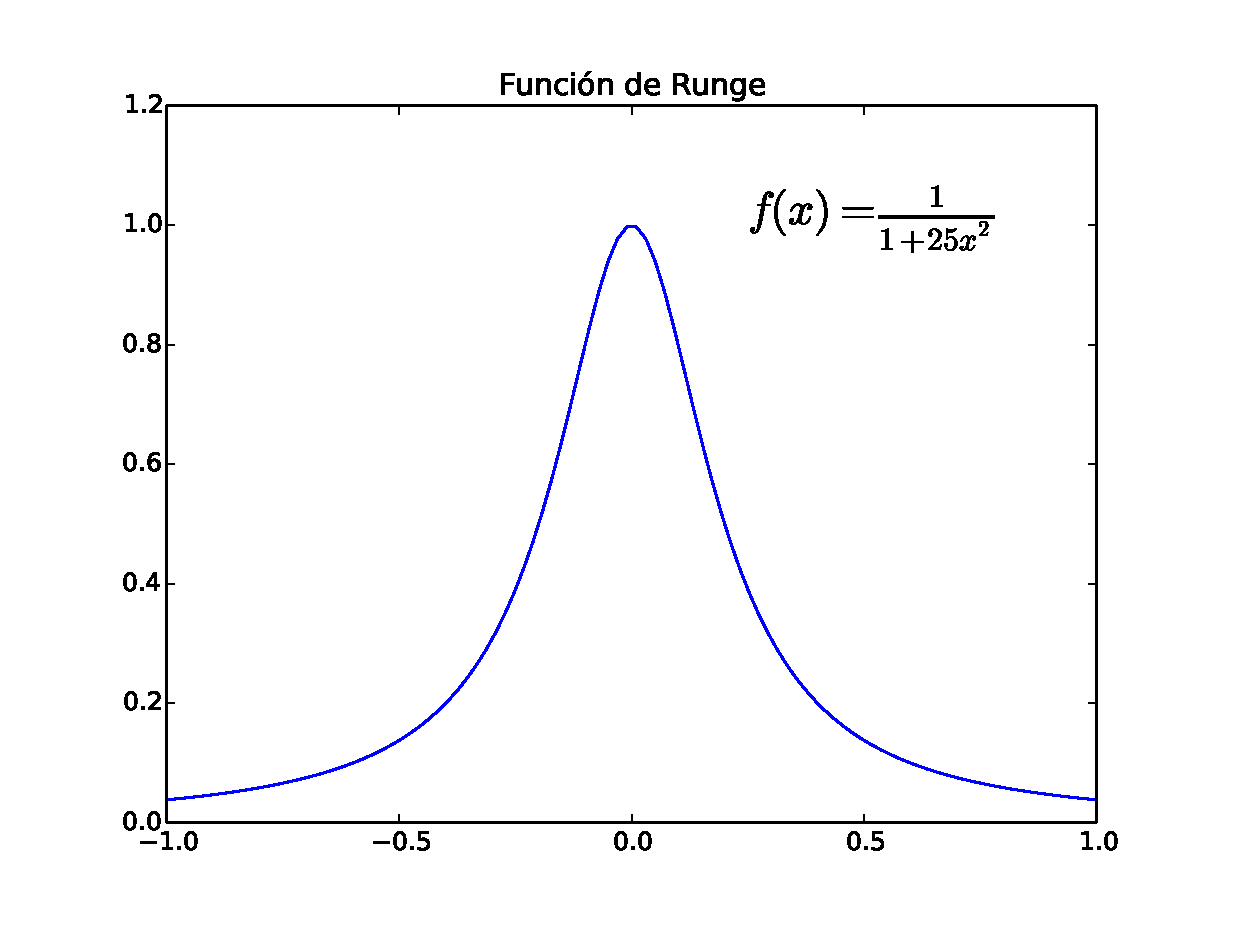
\includegraphics[scale=0.47]{Imagenes/Funcion_Runge_01.eps} 
\end{figure}
\end{frame}
\begin{frame}
\frametitle{Elección de puntos para interpolar}
\begin{figure}
	\centering
	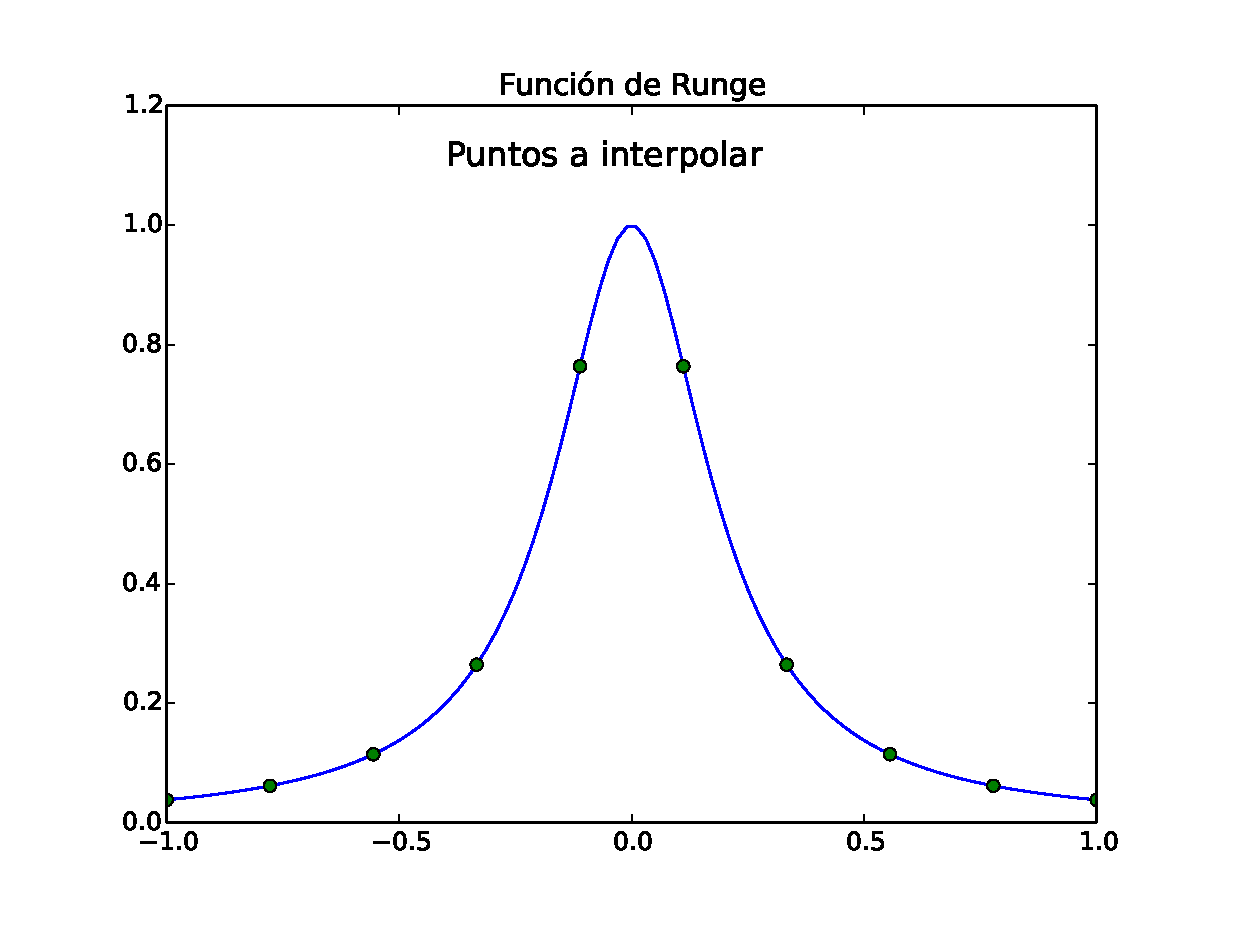
\includegraphics[scale=0.47]{Imagenes/Funcion_Runge_02.eps} 
\end{figure}
\end{frame}
\begin{frame}
\frametitle{Interpolando con el método de Lagrange}
\begin{figure}
	\centering
	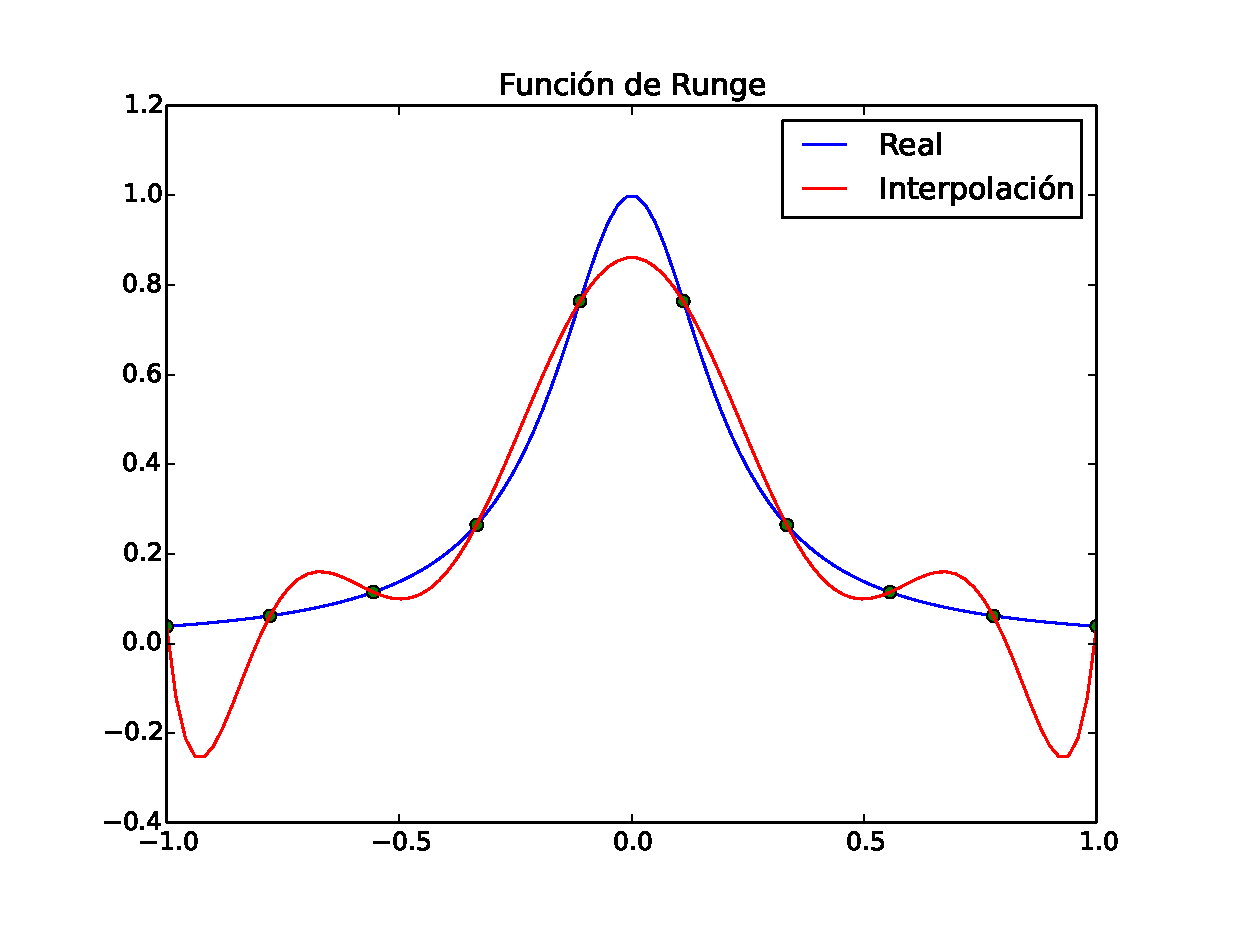
\includegraphics[scale=0.45]{Imagenes/Funcion_Runge_03.eps} 
\end{figure}
\end{frame}
\begin{frame}
\frametitle{¿Qué hacemos al respecto?}
Como hemos visto en la gráfica anterior, la función que resulta del proceso de interpolación \enquote{oscila} a través de los puntos que deseamos interpolar; aquí el caso es que si aumentamos el grado del polinomio, los resultados serán aún más indeseables.
\\
\medskip
\pause
La pregunta obligada es: \textbf{¿qué podemos hacer para mejorar la interpolación?}
\end{frame}

\section{Uso de splines}
\frame{\tableofcontents[currentsection, hideothersubsections]}
\subsection{Definición}

\begin{frame}
\frametitle{¿Qué es un spline?}
En términos nada riguroso, se puede decir que un \textcolor{blue}{spline} es una función definida por una familia de polinomios \enquote{sociables}
\\
\bigskip
\pause
Donde el término \textit{sociable} se usa para indicar que los polinomios que constituyen una función \textcolor{blue}{spline}, están estrechamente vinculados.
\end{frame}
\begin{frame}
\frametitle{El nomobre de spline}    
El nombre de \textcolor{blue}{spline}, viene del inglés ya que es un instrumento que utilizaban los ingenieros navales para dibujar curvas suaves, forzadas a pasar por un conjunto de puntos prefijados.
\end{frame}
\begin{frame}
\frametitle{Las tres B's de los splines}
El uso de las funciones splines tiene mucha aceptación y popularidad se deben a tres razones básicas:
\pause
\setbeamercolor{item projected}{bg=beige,fg=black}
\setbeamertemplate{enumerate items}{%
\usebeamercolor[bg]{item projected}%
\raisebox{1.5pt}{\colorbox{bg}{\color{fg}\footnotesize\insertenumlabel}}%
}
\begin{enumerate}[<+->]
\item \textbf{Buenos:} Se  pueden usar en la solución de una gran variedad de problemas.
\item \textbf{Bonitos:} La teoría matemática en que se basan es muy simple y a la vez elegante.
\item \textbf{Baratos:} Su cálculo es muy sencillo y económico.
\end{enumerate}
\end{frame}
\begin{frame}
\frametitle{Manejando splines con \python}
Usaremos la librería \funcionazul{scipy} que contiene varias funciones con las que ahorramos tiempo para manejar splines y ajustar funciones sociables a un conjunto de datos.
\\
\medskip
\pause
No está de más que revises la teoría al respecto, en la mayoría de los libros de análisis numérico, podrás encontrar la construcción matemática y formal de los splines.
\end{frame}
\begin{frame}
\frametitle{Funciones para los splines}
Necesitaremos de dos pasos para el uso de splines con \python, de la libería: \funcionazul{scipy.interpolate}, las cuales son:
\pause
\setbeamercolor{item projected}{bg=lilac,fg=white}
\setbeamertemplate{enumerate items}{%
\usebeamercolor[bg]{item projected}%
\raisebox{1.5pt}{\colorbox{bg}{\color{fg}\footnotesize\insertenumlabel}}%
}
\begin{enumerate}[<+->]
\item \funcionazul{splrep}: Calcula el spline básico (B-spline) para una curva 1-D.
\\
\medskip
Dados un conjunto de puntos $(x[i],y[i])$ determina una aproximación con un spline suave de grado $k$ en el intervalo $xb \leq x \leq xe$.
\seti
\end{enumerate}
\end{frame}
\begin{frame}
\frametitle{Funciones para los splines}
\setbeamercolor{item projected}{bg=lilac,fg=white}
\setbeamertemplate{enumerate items}{%
\usebeamercolor[bg]{item projected}%
\raisebox{1.5pt}{\colorbox{bg}{\color{fg}\footnotesize\insertenumlabel}}%
}
\begin{enumerate}[<+->]
\conti    
\item \textbf{splev}: Evalúa un B-spline o sus derivadas. Dados los nodos y coeficientes de un B-spline, calcula 
el valor del polinomio suave y sus derivadas.
\end{enumerate}
\end{frame}
\begin{frame}[allowframebreaks, fragile]
\frametitle{Código}
\begin{lstlisting}
import matplotlib.pyplot as plt
import scipy.interpolate as si
from numpy import linspace

def trazador_cub(n):
    xi = linspace(-1, 1, n)
    yi = 1./(1 + 25*xi**2)
    tck = si.splrep(xi, yi)
    return tck

x = linspace(-1, 1, 100)
y = 1./(1 + 25*x**2)

tck = trazador_cub(8)
ys8 = si.splev(x, tck)

tck = trazador_cub(12)
ys12 = si.splev(x, tck)

plt.plot(x, y)
plt.plot(x, ys8,'+g-', label='n=8')
plt.plot(x, ys12,'+r-',label ='n=12')
plt.legend(loc='best')
plt.title('Interpolacion con splines cubicos')
plt.ylim(-0.2, 1.2)
plt.show()
\end{lstlisting}
\end{frame}
\begin{frame}
\frametitle{Resultados gráficos}
\begin{figure}
	\centering
	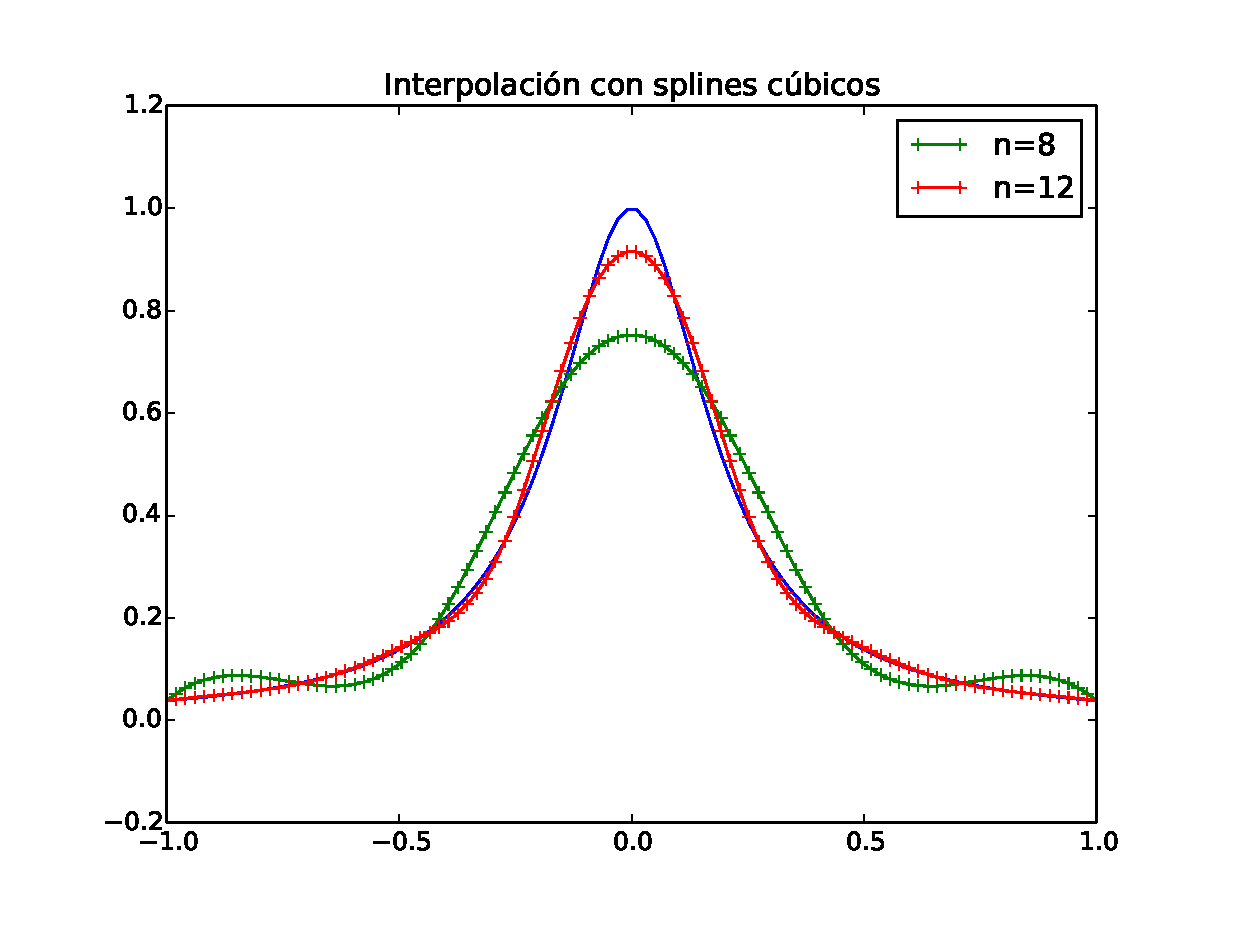
\includegraphics[scale=0.47]{Imagenes/Funcion_Runge_04.eps} 
\end{figure}
\end{frame}
\end{document}
